\documentclass[a4paper]{article}
\usepackage{ctex}
\usepackage{amsmath, amssymb, amsthm}
\usepackage{moreenum}
\usepackage{mathtools}
\usepackage{url}
\usepackage{bm}
\usepackage{enumitem}
\usepackage{graphicx}
\usepackage{listings}
\usepackage{color}

\usepackage{fontspec}
\usepackage{xcolor}

\usepackage{float}

\definecolor{codekeyword}{RGB}{171, 0, 216}
\definecolor{codetypename}{RGB}{29, 37, 251}
\definecolor{codevariable}{RGB}{10, 23, 126}
\definecolor{codestring}{RGB}{157, 0, 25}
\definecolor{codecomment}{RGB}{31, 129, 19}
\definecolor{codebackground}{RGB}{230 235 245}

\newfontfamily\cascadia[Ligatures=ResetAll]{Cascadia Code}

\lstset{
    basicstyle          =   \footnotesize\cascadia,          % 基本代码风格
    keywordstyle        =   \bfseries,          % 关键字风格
    commentstyle        =   \rmfamily\itshape,  % 注释的风格,斜体
    stringstyle         =   \ttfamily,  % 字符串风格
    flexiblecolumns,                % 别问为什么,加上这个
    numbers             =   left,   % 行号的位置在左边
    showspaces          =   false,  % 是否显示空格,显示了有点乱,所以不现实了
    numberstyle         =   \cascadia,    % 行号的样式,小五号,tt等宽字体
    showstringspaces    =   false,
    captionpos          =   t,      % 这段代码的名字所呈现的位置,t指的是top上面
    backgroundcolor     =   \color{codebackground},
    breaklines          =   true,
    frame               =   l,
}

\lstdefinestyle{Python}{
    language        =   Python, % 语言选Python
    basicstyle      =   \zihao{-5}\ttfamily,
    numberstyle     =   \zihao{-5}\ttfamily,
    keywordstyle    =   \color{blue},
    keywordstyle    =   [2] \color{teal},
    stringstyle     =   \color{magenta},
    commentstyle    =   \color{red}\ttfamily,
    breaklines      =   true,   % 自动换行,建议不要写太长的行
    columns         =   fixed,  % 如果不加这一句,字间距就不固定,很丑,必须加
    basewidth       =   0.5em,
}
\usepackage{subcaption}
\usepackage{booktabs} % toprule
\usepackage[mathcal]{eucal}
\usepackage[thehwcnt = 2]{iidef}

\usepackage{pdfpages}

\setenumerate[1]{label=(\arabic{*})}
\setenumerate[2]{label=\arabic{*})}


\thecourseinstitute{清华大学电子工程系}
\thecoursename{\textbf{媒体与认知}}
\theterm{2023-2024学年春季学期}
\hwname{作业}
\begin{document}
\courseheader
% 请在YOUR NAME处填写自己的姓名
\name{毕嘉仪 2022010608}
\vspace{3mm}
\centerline{\textbf{\Large{理论部分}}}

\section{单选题(15分)}
% 请在?处填写答案
\subsection{\underline{D}}

\subsection{\underline{C}}

\subsection{\underline{D}}

\subsection{\underline{D}}

\subsection{\underline{B}}
\clearpage

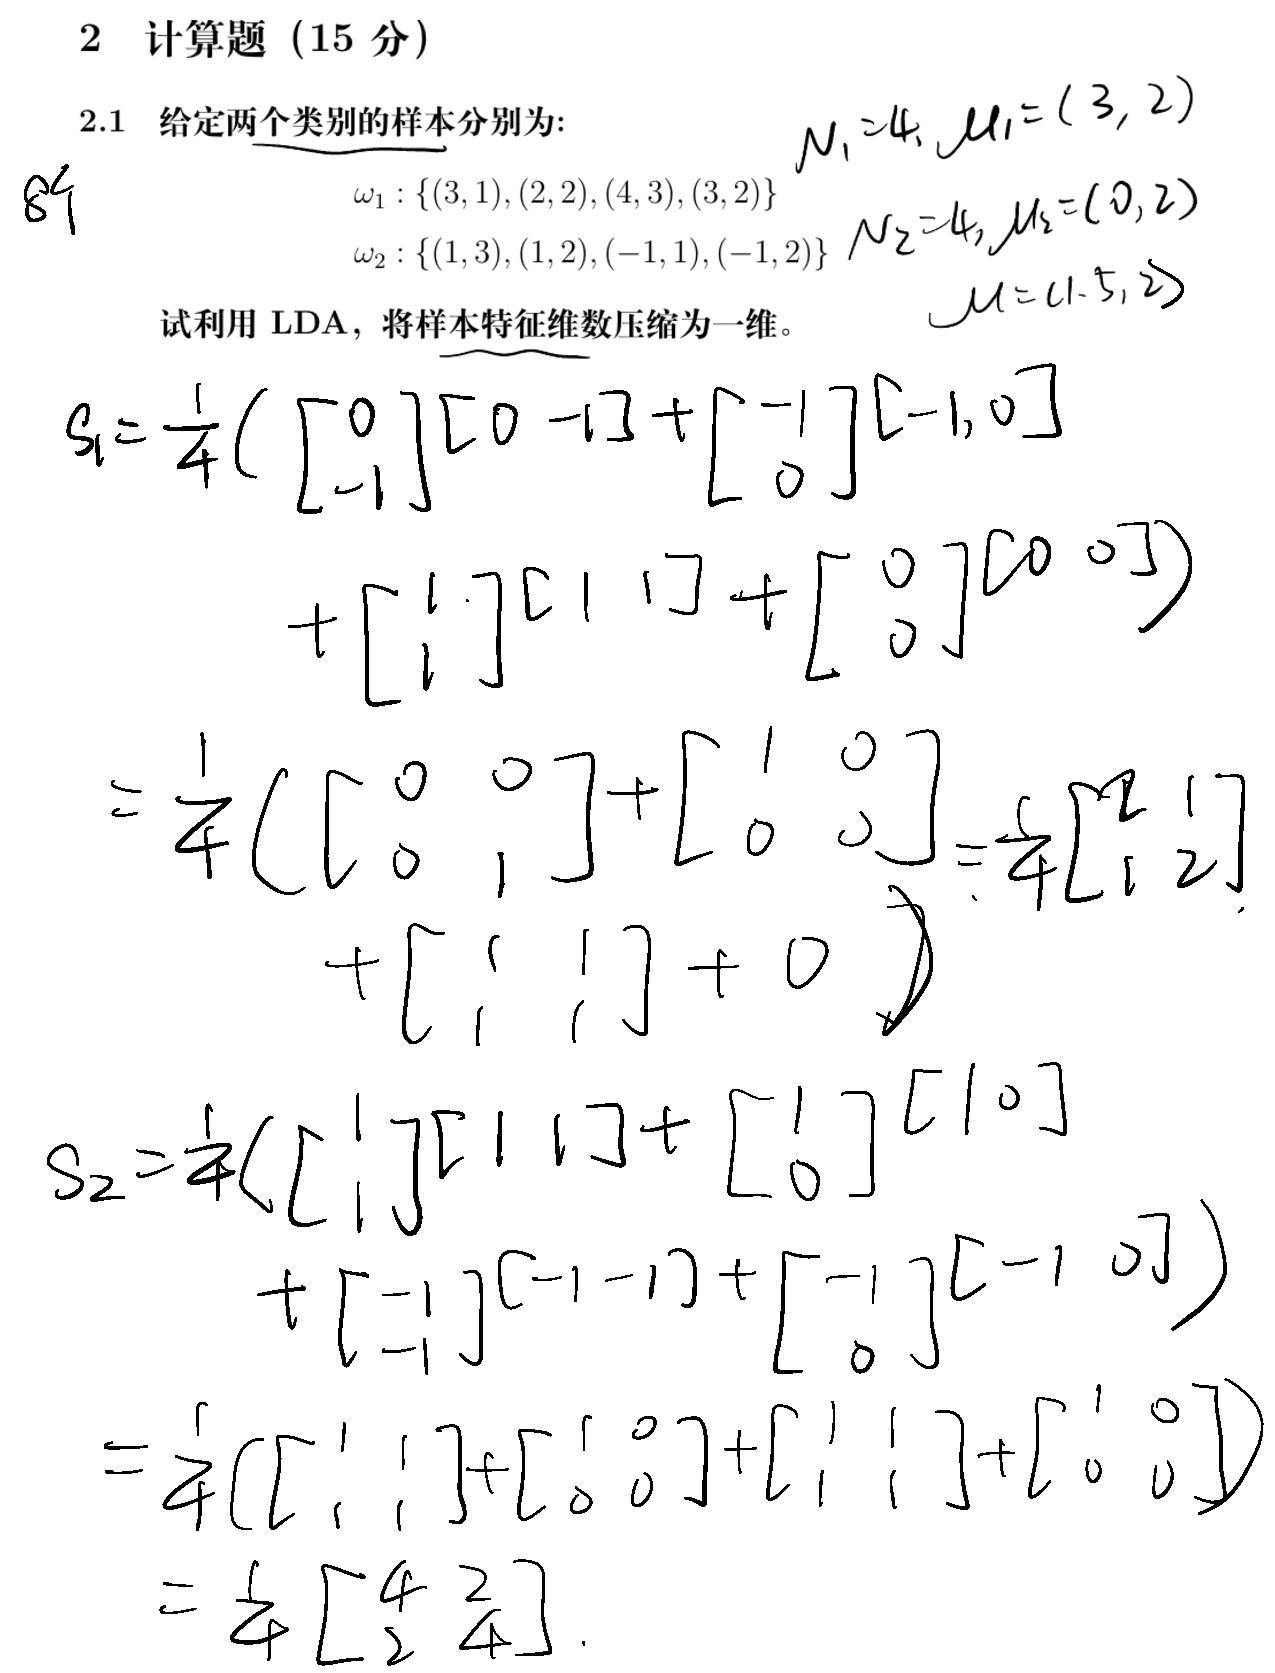
\includepdf[pages=-, scale=0.8, pagecommand={}]{myHW3.pdf}


\vspace{3mm}
\centerline{\textbf{\Large{编程部分}}}
% 请根据是否选择自选课题的情况选择“编程作业报告”或“自选课题进度汇报”中的一项完成
\section{编程作业报告}
% 请在此处完成编程作业报告
\subsection{程序验证}
输入:
\lstinputlisting{../../file/1_in.txt}
结果图像:
\begin{figure}[H]
    \centering
    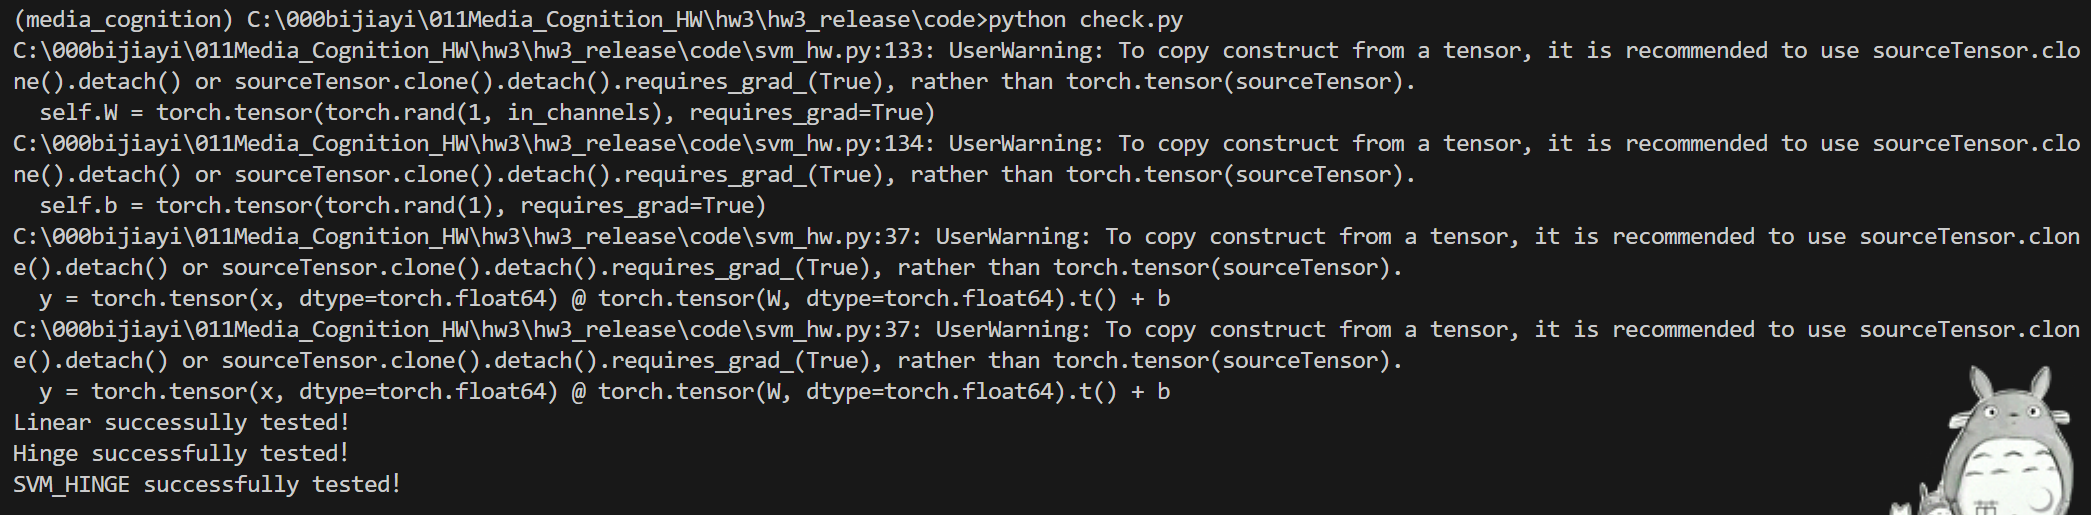
\includegraphics[width=0.9\linewidth]{../../img/checkSVM-result.png}
\end{figure}

\subsection{数据预处理}
输入:
\lstinputlisting{../../file/2_in.txt}
可视化结果:
\begin{figure}[H]
    \centering
        \begin{subfigure}[b]{.45\linewidth}
            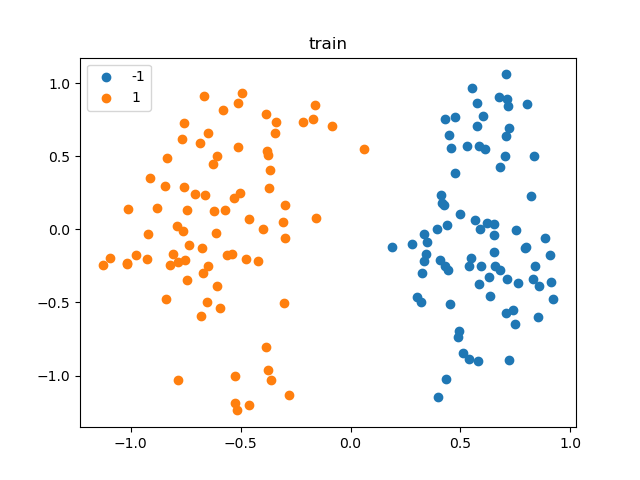
\includegraphics[width=\linewidth]{../../img/pca-train.png}
        \end{subfigure}
        \begin{subfigure}[b]{.45\linewidth}
            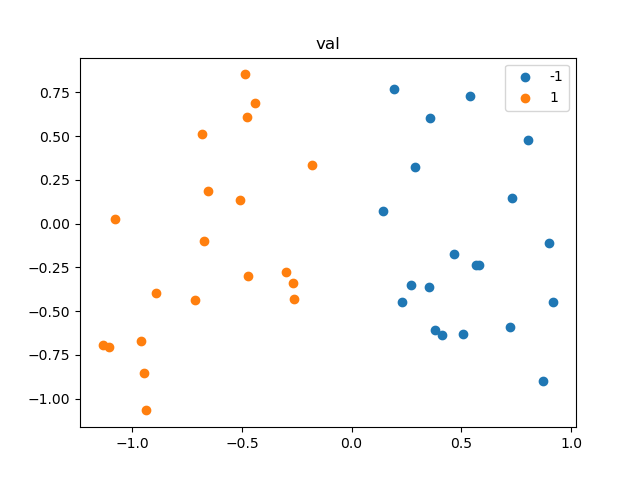
\includegraphics[width=\linewidth]{../../img/pca-val.png}
        \end{subfigure}
        \begin{subfigure}[b]{.45\linewidth}
            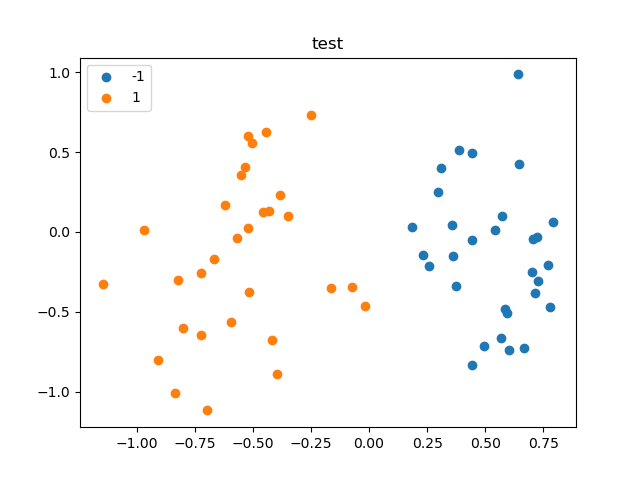
\includegraphics[width=\linewidth]{../../img/pca-test.png}
        \end{subfigure}
\end{figure}

\subsection{训练、验证及测试}
\begin{enumerate}
    \item 训练模型
    
    输入:
    \lstinputlisting{../../file/3_1_in.txt}
    输出:
    \begin{figure}[H]
        \centering
	        \begin{subfigure}[b]{.45\linewidth}
	            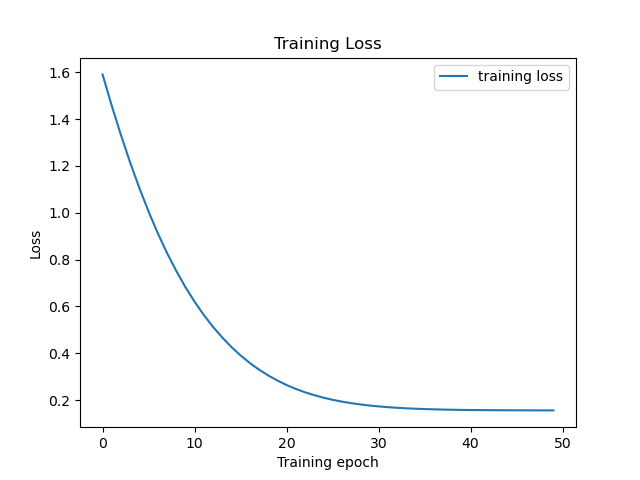
\includegraphics[width=\linewidth]{../../img/3-1.png}
	        \end{subfigure}
	        \begin{subfigure}[b]{.45\linewidth}
	            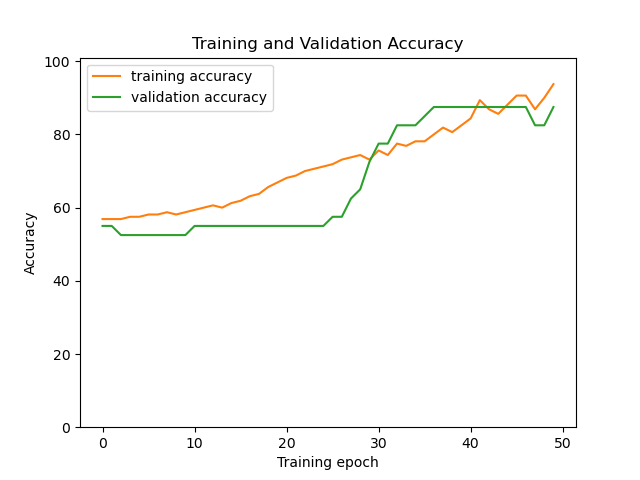
\includegraphics[width=\linewidth]{../../img/3-2.png}
	        \end{subfigure}
	        \begin{subfigure}[b]{.45\linewidth}
	            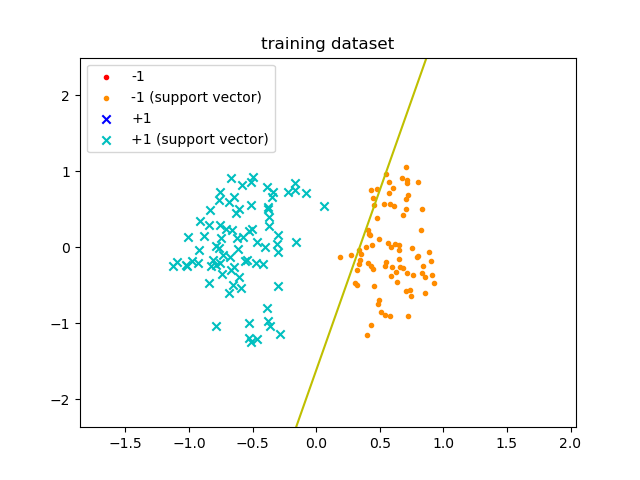
\includegraphics[width=\linewidth]{../../img/3-3.png}
	        \end{subfigure}
	        \begin{subfigure}[b]{.45\linewidth}
	            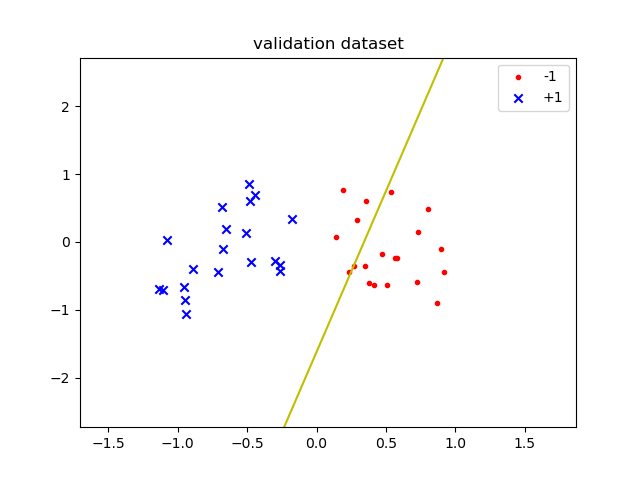
\includegraphics[width=\linewidth]{../../img/3-4.png}
	        \end{subfigure}
    \end{figure}

    \item 测试模型
    
    输入:
    \lstinputlisting{../../file/3_2_in.txt}

    输出:
    \lstinputlisting{../../file/3_2_out.txt}
\end{enumerate}

\subsection{调整正则化系数$C$,分析不同的$C$值对分类效果的影响。}
\begin{enumerate}
    \item 分别输入:
    
    \lstinputlisting{../../file/4_in.txt}
    
    图像输出见下:
    \begin{enumerate}
        \item $C = 1e-6$
        \begin{figure}[H]
            \centering
                \begin{subfigure}[b]{.45\linewidth}
                    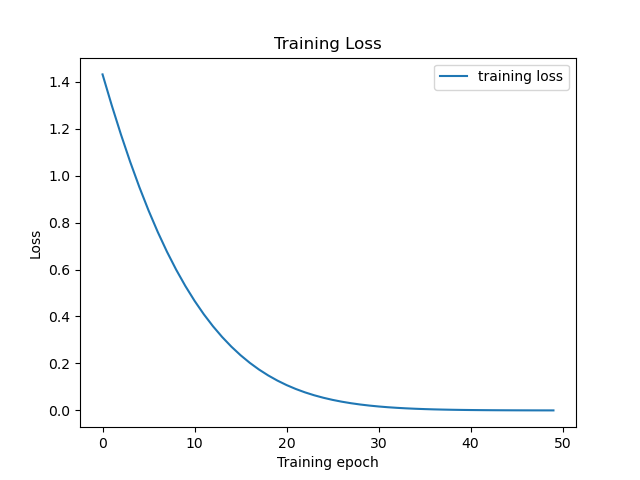
\includegraphics[width=\linewidth]{../../img/4-1-1.png}
                \end{subfigure}
                \begin{subfigure}[b]{.45\linewidth}
                    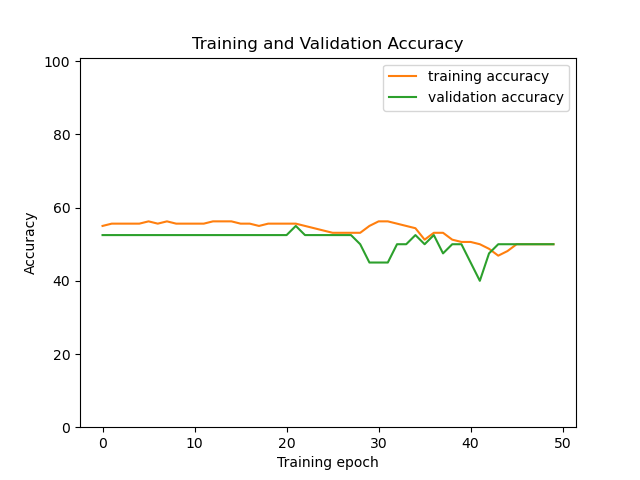
\includegraphics[width=\linewidth]{../../img/4-1-2.png}
                \end{subfigure}
                \begin{subfigure}[b]{.45\linewidth}
                    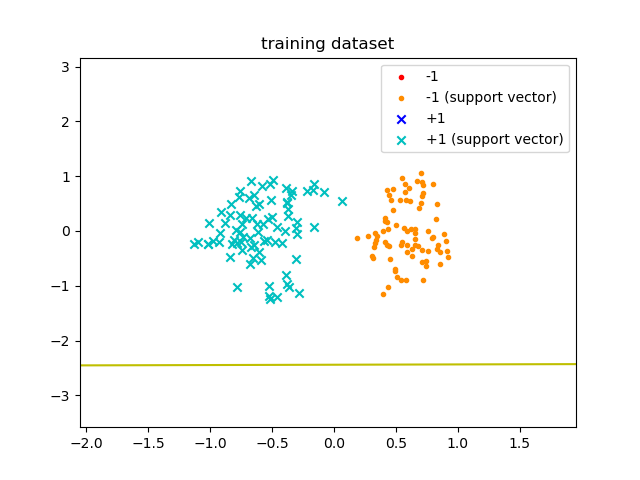
\includegraphics[width=\linewidth]{../../img/4-1-3.png}
                \end{subfigure}
                \begin{subfigure}[b]{.45\linewidth}
                    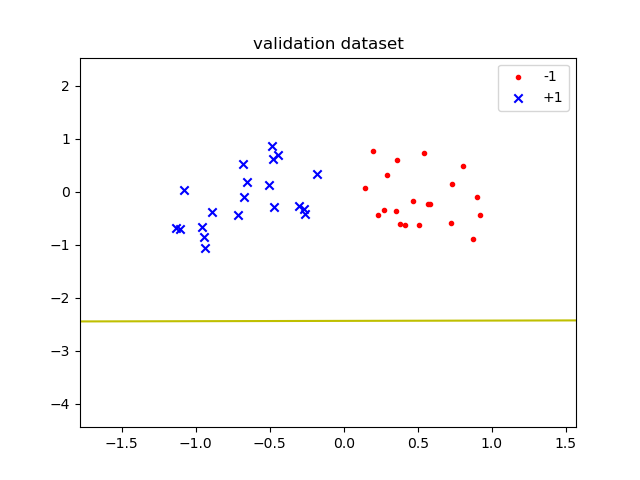
\includegraphics[width=\linewidth]{../../img/4-1-4.png}
                \end{subfigure}
        \end{figure}

        \item $C = 1e-3$
        \begin{figure}[H]
            \centering
                \begin{subfigure}[b]{.45\linewidth}
                    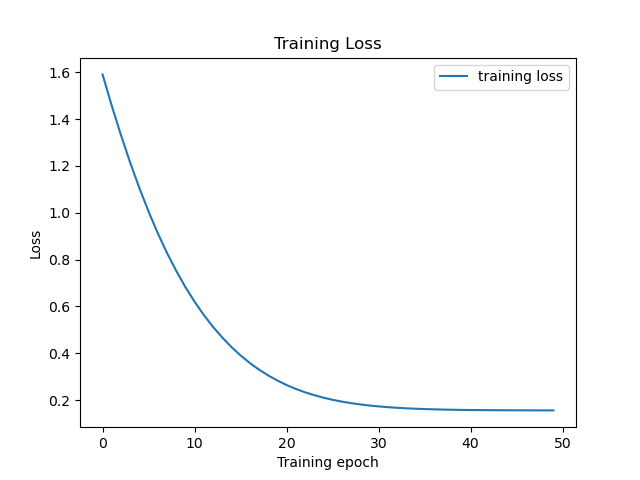
\includegraphics[width=\linewidth]{../../img/3-1.png}
                \end{subfigure}
                \begin{subfigure}[b]{.45\linewidth}
                    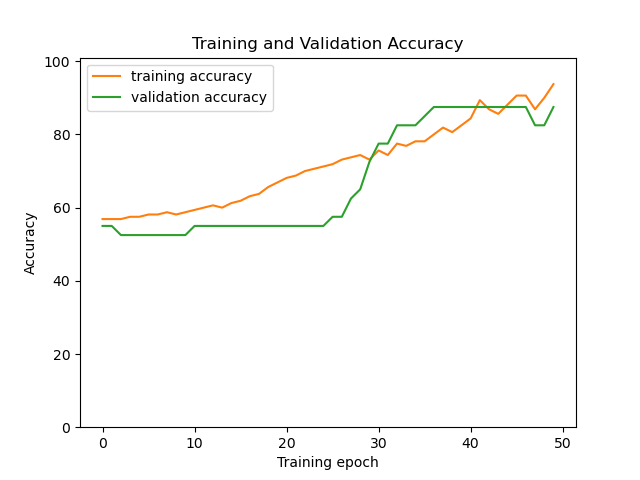
\includegraphics[width=\linewidth]{../../img/3-2.png}
                \end{subfigure}
                \begin{subfigure}[b]{.45\linewidth}
                    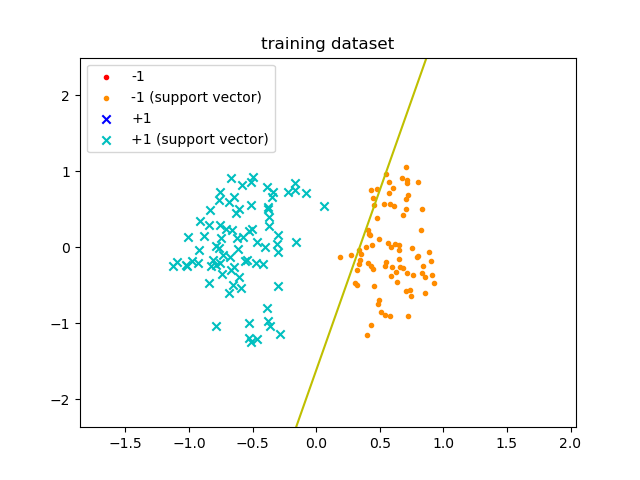
\includegraphics[width=\linewidth]{../../img/3-3.png}
                \end{subfigure}
                \begin{subfigure}[b]{.45\linewidth}
                    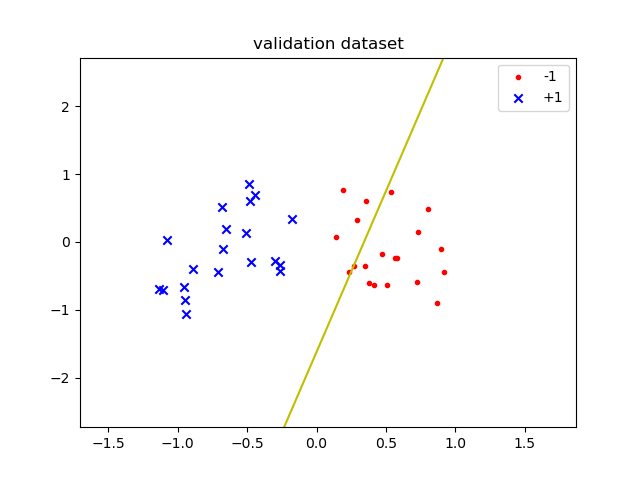
\includegraphics[width=\linewidth]{../../img/3-4.png}
                \end{subfigure}
        \end{figure}
        
        \item $C = 1$
        \begin{figure}[H]
            \centering
                \begin{subfigure}[b]{.45\linewidth}
                    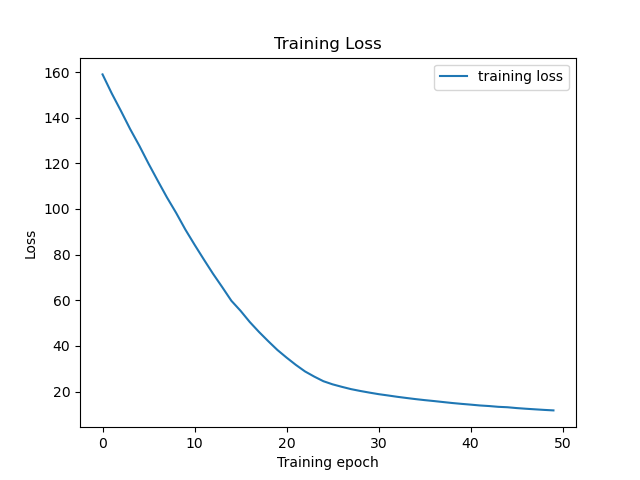
\includegraphics[width=\linewidth]{../../img/4-3-1.png}
                \end{subfigure}
                \begin{subfigure}[b]{.45\linewidth}
                    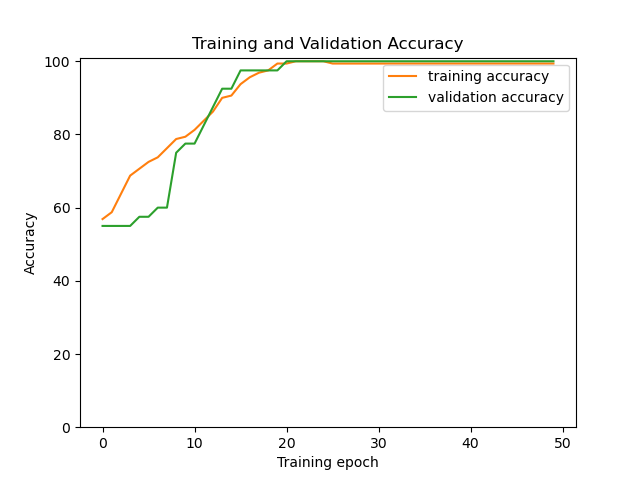
\includegraphics[width=\linewidth]{../../img/4-3-2.png}
                \end{subfigure}
                \begin{subfigure}[b]{.45\linewidth}
                    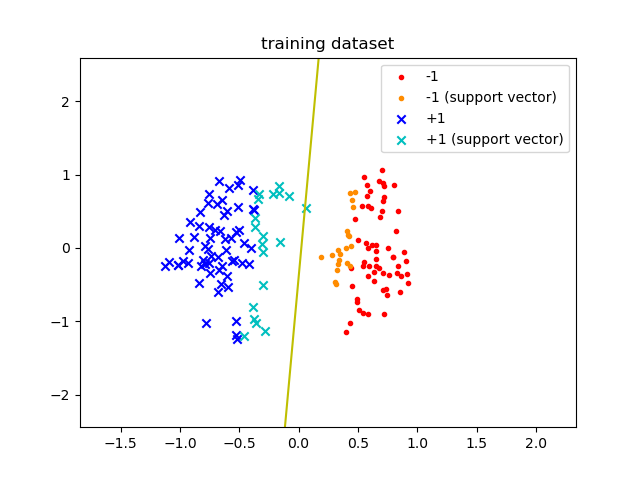
\includegraphics[width=\linewidth]{../../img/4-3-3.png}
                \end{subfigure}
                \begin{subfigure}[b]{.45\linewidth}
                    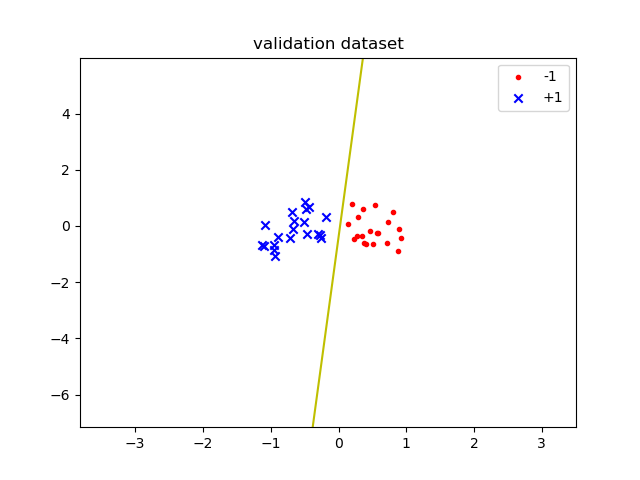
\includegraphics[width=\linewidth]{../../img/4-3-4.png}
                \end{subfigure}
        \end{figure}
        
    \end{enumerate}

    测试准确率输出分别如下:
    \lstinputlisting{../../file/4_out.txt}

    \item 分析

    $C$越大,即要求模型的误差越小,进入间隔区间的点越少,容易过拟合;$C$越小,即模型的误差越大,进入间隔区间的点越多,训练集上容易出现欠拟合。
\end{enumerate}

\end{document}



%%% Local Variables:
%%% mode: late\rvx
%%% TeX-master: t
%%% End:
